\documentclass[11pt]{article}
\usepackage[margin=0.88in]{geometry}
\usepackage[T1]{fontenc}
\usepackage[utf8]{inputenc}
\usepackage{microtype}
\usepackage{graphicx}
\usepackage{booktabs}
\usepackage{array}
\usepackage{tabularx}
\usepackage{float}
\usepackage{amsmath}
\usepackage{hyperref}
\graphicspath{{figures/}}
\hypersetup{colorlinks=true,linkcolor=blue,urlcolor=blue,pdftitle={Supplementary material: Qualifying Image-Grounded Tag Retrieval in Piping and Instrumentation Diagrams with Source-Isolated Counterfactual Evaluation}}
\setlength{\emergencystretch}{3em}
\newcolumntype{Y}{>{\raggedright\arraybackslash}X}
\newcolumntype{P}[1]{>{\raggedright\arraybackslash}p{#1}}

\title{Supplementary material: Qualifying Image-Grounded Tag Retrieval in Piping and Instrumentation Diagrams with Source-Isolated Counterfactual Evaluation}
\author{Author names and affiliations to be supplied at submission}
\date{}

\begin{document}
\maketitle

\section*{S1. Positioning and evidence contract}

The manuscript evaluates a bounded engineering decision: whether a specified
model and visual-input budget support candidate-tag retrieval on unseen source
drawings. It does not propose a new recognition architecture or claim complete
P\&ID digitization. Table~S1 distinguishes the contribution from adjacent
work using only dimensions relevant to that decision.

\begin{table}[H]
\centering
\caption{Positioning relative to representative P\&ID and document-VQA work.
Bibliographic details and DOIs appear in the main manuscript.}
\label{tab:s1_position}
\scriptsize
\begin{tabularx}{\linewidth}{P{0.18\linewidth}P{0.22\linewidth}P{0.20\linewidth}P{0.17\linewidth}Y}
\toprule
Work & Primary input/domain & Primary output & Evaluation emphasis & Relation to this study \\
\midrule
Paliwal et al. (2021) & Synthetic P\&ID images & Digitized diagram elements & End-to-end digitization pipeline & Source resource and broader digitization target \\
Kim et al. (2021) & High-density industrial P\&ID images & Symbols and text & Industrial recognition performance & Demonstrates specialized recognition beyond generic VLM prompting \\
Su et al. (2024) & High-resolution industrial P\&ID images & Symbols, text, and pipelines & Multi-stage visual recognition & Motivates task-specific rather than aggregate evaluation \\
Gupta et al. (2025) & 500 Dataset-PID sheets & 64,000 graph-derived QA records & P\&ID question answering & Dataset and task taxonomy used here \\
Nourbakhsh et al. (2025) & Document VQA & Grounding-aware evaluation & Whether outputs are attributable to documents & Adjacent grounding motivation \\
This study & Source-isolated PIDQA drawings & Candidate value-tag sets & Correct, shuffled, and absent images; budget and scope gates & Evaluation and qualification workflow \\
\bottomrule
\end{tabularx}
\end{table}

The evidence phases are:
\begin{enumerate}
\item configuration records, used to freeze prompt, parser, legal tag grammar,
and inference conditions;
\item primary Set B qualification, using 100 unseen source drawings;
\item descriptive Set B fusion, where the component predictions motivated a
complete four-rule operating family;
\item frozen-rule within-family checks on seed-29/31 partitions, followed by
explicit source-overlap exclusions.
\end{enumerate}
The last phase is stability evidence inside PIDQA, not an external replication.

\section*{S2. Frozen prompts, parsing, and answer isolation}

The exact Qwen P0 template is:

\begin{quote}\small\ttfamily\raggedright
You analyze a piping and instrumentation diagram (P\&ID). Answer only from the
visible diagram. Return only the final answer, without explanation or
Markdown.\\[2pt]
Question: \{question\}
\end{quote}

The matched InternVL prompt uses the same sentence sequence. Image conditions
prepend the model's \texttt{<image>} placeholder; the no-image condition does
not. All generation is greedy. Qwen rows record maximum image side and output
cap separately. InternVL image rows record realised 448-pixel tiles and output
cap. The tokenizer-corrected InternVL pass sets
\texttt{fix\_mistral\_regex=true}; the warned diagnostic pass is retained in
the archive but is not used for reported scores.

Strict value scoring lowercases, trims, de-duplicates, sorts, and compares tag
sets. The conservative grammar accepts alphabetic prefixes followed by
numeric, hyphen-numeric, or space-numeric suffixes (for example
\texttt{KL-58999}, \texttt{UV-00-001}, \texttt{SDL 299}, and
\texttt{CV1}); bare uppercase tags are accepted after a frozen stopword
filter. Empty strings and \texttt{[]} map to an empty set. The parser never
reads the hidden reference.

The answer-isolation audit covers seven public manifests and 13 primary E2--E8
raw output files. Every successful output's legacy \texttt{answer} field
aliases generated \texttt{raw} text rather than a reference label. Scorer-
only references are used after inference for evaluation and for no prediction
construction.

\section*{S3. Estimator and uncertainty definitions}

For source $i$, let $T_i$ and $P_i$ be reference and prediction sets. The
element counts are
\[
TP_i=|T_i\cap P_i|,\qquad FP_i=|P_i\setminus T_i|,\qquad
FN_i=|T_i\setminus P_i|.
\]
Micro precision and recall pool the counts across sources, and pooled F1 is
\[
F1_{\mathrm{micro}}=
\frac{2\sum_iTP_i}{2\sum_iTP_i+\sum_iFP_i+\sum_iFN_i}.
\]
Source-macro quantities compute precision, recall, and F1 separately for each
source and average each metric over sources. Exact-set accuracy is the source
mean of the indicator that $T_i=P_i$.

When $T_i=P_i=\emptyset$, the per-source precision, recall, and F1 are set to
1 because the source is exactly resolved. When $T_i\neq\emptyset$ and
$P_i=\emptyset$, all three are 0. Seven of 100 Set B value sources have empty
references. To make the convention visible, all-source macro and
non-empty-reference macro values are reported together.

Intervals are 95\% percentile intervals from 10,000 source bootstrap
replicates. Paired comparisons resample the same source indices for both
conditions. Random numbers use \path{numpy.random.default_rng} (PCG64), with
fixed comparison-specific seeds recorded in
\path{rineng_revision_analysis_v6.json}. No record-level interval and no
post-observation equivalence margin are used.

\section*{S4. Source splitting and aggregate boundary}

The input-retrieval-plus-prior diagnostic uses exact image SHA-256 plus a
released-template semantic signature and a training-only task-majority
fallback. It uses no learned embedding, nearest-neighbour search, or
\texttt{source\_id} cache key. Each split has 38,400 training and 12,800 test
questions; the 20\% calibration partition is unused.

\begin{table}[H]
\centering
\caption{All five pre-specified split diagnostics.}
\label{tab:s4_split}
\small
\begin{tabular}{rrrrr}
\toprule
Seed & Question-random & Source-isolated & Difference & Difference (points) \\
\midrule
3 & 0.5199 & 0.3128 & +0.2071 & +20.71 \\
17 & 0.5253 & 0.3121 & +0.2132 & +21.32 \\
29 & 0.5248 & 0.3148 & +0.2101 & +21.01 \\
43 & 0.5217 & 0.3141 & +0.2077 & +20.77 \\
71 & 0.4554 & 0.3194 & +0.1360 & +13.60 \\
\midrule
Mean & 0.5094 & 0.3146 & +0.1948 & +19.48 \\
\bottomrule
\end{tabular}
\end{table}

The independent training-only task-majority diagnostic scores 0.3375 aggregate
strict accuracy on Set B. Correct-image Qwen aggregate strict accuracy is
0.2875 and no-image accuracy is 0.3025. These are not tag F1 values; they are
reported to show why aggregate benchmark accuracy does not qualify image-
grounded retrieval.

\section*{S5. Qwen counterfactual and budget controls}

\begin{table}[H]
\centering
\caption{Value-tag controls. Effects are paired source-level pooled-F1
differences with 10,000 source-bootstrap replicates.}
\label{tab:s5_controls}
\small
\begin{tabular}{lrrr}
\toprule
Contrast & Baseline F1 & Condition F1 & Difference [95\% interval] \\
\midrule
3072 minus 768, 192-token cap & 0.0000 & 0.5549 & +0.5549 [0.4774, 0.6314] \\
3072 minus 768, 512-token cap & 0.0003 & 0.5253 & +0.5250 [0.4224, 0.6293] \\
Correct minus source-shuffled, 3072/192 & 0.0062 & 0.5549 & +0.5487 [0.4729, 0.6239] \\
Correct minus no image, 3072/192 & 0.0000 & 0.5549 & +0.5549 [0.4799, 0.6322] \\
\bottomrule
\end{tabular}
\end{table}

\begin{table}[H]
\centering
\caption{Recorded operating quantities. Tensor elements are processor
outputs, not asserted visual-token counts. Peak memory is observed allocated
memory on the H200 run.}
\label{tab:s5_budget}
\scriptsize
\resizebox{\linewidth}{!}{%
\begin{tabular}{lrrrrrr}
\toprule
Condition & Actual input & Cap & Tokens mean & Tokens p95 & Cap rate & Peak GiB \\
\midrule
Qwen 768 correct, value & 2,211,840 elements & 512 & 421.2 & 512 & 79.0\% & 16.50 \\
Qwen 3072 correct, value & 35,979,264 elements & 512 & 54.7 & 512 & 6.0\% & 18.17 \\
InternVL one tile, all tasks & 1 / 602,112 elements & 192 & 51.0 & 192 & 17.8\% & 16.04 \\
InternVL seven tiles, all tasks & 7 / 4,214,784 elements & 192 & 16.4 & 63 & 2.8\% & 17.41 \\
\bottomrule
\end{tabular}}
\end{table}

For the matched Qwen comparison, the processor-element ratio is 16.27. The
768-side condition generates substantially longer text and reaches the cap
more often. End-to-end latency is therefore not interpreted as isolated
visual-encoder cost. Legacy 192-token Qwen rows lack processor-element and
peak-allocation telemetry; these values are not back-filled.

\begin{figure}[H]
\centering
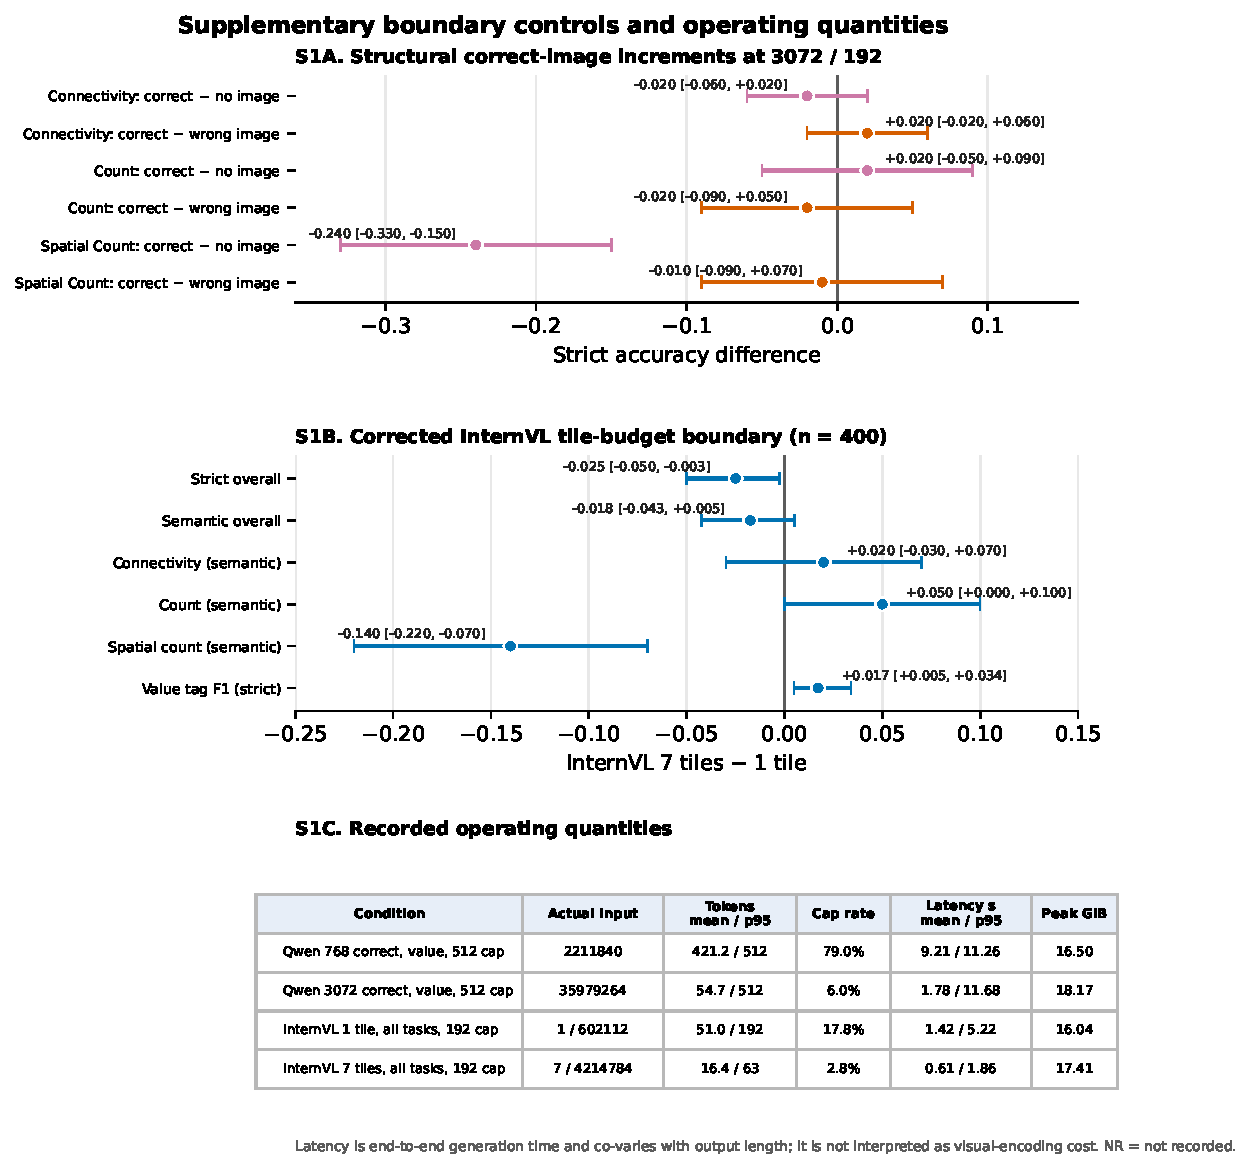
\includegraphics[width=\linewidth]{figure_s1_controls_and_operating_quantities_v4.pdf}
\caption{Structural correct-image increments, corrected InternVL tile-budget
boundary, and recorded operating quantities. This boundary figure is retained
in the supplement so that the main tag-retrieval claim is not generalized to
all tasks or model families.}
\label{fig:s1_controls}
\end{figure}

\section*{S6. OCR literal-versus-join ablation}

PaddleOCR processes the complete source drawing with the English PP-OCRv3
detector and PP-OCRv4 recognizer, CPU execution, no crop, no angle classifier,
and detector maximum side 3072. The geometry rule joins a recognized
alphabetic prefix to the nearest vertically stacked numeric fragment within
frozen distance limits. Fully formed tags with final numeric segments longer
than two characters are never extended. Coordinates and grammar are used;
references are not.

\begin{table}[H]
\centering
\caption{OCR parsing ablation on the same 100 Set B value sources.}
\label{tab:s6_ocr}
\small
\begin{tabular}{lrrrrrrrr}
\toprule
Parse & TP & FP & FN & Precision & Recall & Micro F1 & Macro F1 & Exact \\
\midrule
Literal & 116 & 44 & 232 & 0.7250 & 0.3333 & 0.4567 & 0.4227 & 0.1200 \\
Geometry join v1 & 159 & 29 & 189 & 0.8457 & 0.4569 & 0.5933 & 0.5618 & 0.2100 \\
\bottomrule
\end{tabular}
\end{table}

There are 45 join operations. Relative to literal parsing, the joined output
adds 44 true tags and one false candidate, removes 16 false candidates and one
true tag, improves per-source F1 on 16 drawings, degrades it on one, and is
unchanged on 83. This is a deterministic normalization ablation; it is not a
claim that every joined string is semantically correct outside the benchmark
grammar.

\section*{S7. Complete operating family, estimators, and workload}

All rules use the fixed Qwen and geometry-joined OCR predicted sets only. No
reference, fitted confidence threshold, or rule re-selection enters a fused
prediction.

\begin{table}[H]
\centering
\caption{Set B components and complete four-rule family. The non-empty macro
column averages only the 93 sources containing at least one reference tag.}
\label{tab:s7_all}
\scriptsize
\resizebox{\linewidth}{!}{%
\begin{tabular}{lrrrrrrrrrr}
\toprule
Mode & TP & FP & FN & P & R & Micro F1 & Macro F1 & Non-empty macro F1 & Exact & Empty predictions \\
\midrule
Qwen & 192 & 152 & 156 & 0.5581 & 0.5517 & 0.5549 & 0.5810 & 0.6139 & 0.1900 & 1 \\
OCR geometry & 159 & 29 & 189 & 0.8457 & 0.4569 & 0.5933 & 0.5618 & 0.5396 & 0.2100 & 18 \\
Set union & 245 & 180 & 103 & 0.5765 & 0.7040 & 0.6339 & 0.6602 & 0.6991 & 0.1900 & 1 \\
Set intersection & 106 & 1 & 242 & 0.9907 & 0.3046 & 0.4659 & 0.4312 & 0.3992 & 0.1700 & 41 \\
OCR if non-empty, else Qwen & 175 & 39 & 173 & 0.8178 & 0.5029 & 0.6228 & 0.6073 & 0.6423 & 0.2200 & 1 \\
Qwen if non-empty, else OCR & 192 & 152 & 156 & 0.5581 & 0.5517 & 0.5549 & 0.5810 & 0.6139 & 0.1900 & 1 \\
\bottomrule
\end{tabular}}
\end{table}

\begin{table}[H]
\centering
\caption{Per-drawing candidate workload, median [IQR]. False candidates are
predicted tags absent from the benchmark reference.}
\label{tab:s7_workload}
\small
\begin{tabular}{lrr}
\toprule
Mode & Candidate count & False-candidate count \\
\midrule
Qwen & 3 [1, 4] & 0 [0, 2] \\
OCR literal & 1 [1, 2] & 0 [0, 1] \\
OCR geometry & 2 [1, 3] & 0 [0, 0] \\
Set union & 4 [2, 5] & 1 [0, 2] \\
Set intersection & 1 [0, 2] & 0 [0, 0] \\
OCR if non-empty, else Qwen & 2 [1, 3] & 0 [0, 1] \\
\bottomrule
\end{tabular}
\end{table}

\begin{table}[H]
\centering
\caption{Selected paired differences on Set B across estimators.}
\label{tab:s7_diffs}
\scriptsize
\begin{tabular}{llrr}
\toprule
Comparison & Estimator & F1 difference & 95\% interval \\
\midrule
Union minus Qwen & Micro pooled & +0.0790 & [0.0372, 0.1261] \\
Union minus Qwen & Source macro & +0.0792 & [0.0373, 0.1250] \\
Union minus Qwen & Non-empty source macro & +0.0852 & [0.0398, 0.1346] \\
Union minus OCR & Micro pooled & +0.0406 & [-0.0282, 0.1118] \\
Union minus OCR & Source macro & +0.0984 & [0.0130, 0.1819] \\
OCR-first minus OCR & Micro pooled & +0.0295 & [0.0051, 0.0590] \\
Intersection minus Qwen & Micro pooled & -0.0890 & [-0.1616, -0.0181] \\
\bottomrule
\end{tabular}
\end{table}

Intersection is not intended to maximize F1; it exchanges coverage for a
shortlist with precision 0.9907 and source-bootstrap interval
[0.9681, 1.0000]. The estimator dependence of union minus OCR is retained
rather than collapsed into a single favourable number.

\section*{S8. Source membership audit and frozen-rule checks}

Set B shares 17 sources with seed 29 and 17 with seed 31. Seed 29 and seed 31
share 20 sources; two sources occur in all three sets. Set B exclusion leaves
83 sources in each check, with 18 sources still common to the two checks. A
second exclusion creates two 65-source subsets that share no source with Set B
or with one another.

\begin{table}[H]
\centering
\caption{Union rule across original, Set-B-excluded, and mutually disjoint
subsets. Original-partition rows reproduce the earlier descriptive scorer;
new exclusion rows use the v6 estimator.}
\label{tab:s8_micro}
\scriptsize
\begin{tabular}{lrrrr}
\toprule
Subset & $n$ & Qwen micro F1 & Union micro F1 & Union--Qwen [95\% interval] \\
\midrule
Original seed 29 & 100 & 0.6783 & 0.7167 & +0.0384 [0.0059, 0.0740] \\
Original seed 31 & 100 & 0.6500 & 0.6918 & +0.0418 [0.0048, 0.0852] \\
Seed 29 excluding Set B & 83 & 0.6717 & 0.7083 & +0.0366 [0.0002, 0.0751] \\
Seed 31 excluding Set B & 83 & 0.6417 & 0.6856 & +0.0440 [0.0021, 0.0920] \\
Seed 29 strictly disjoint & 65 & 0.6587 & 0.6911 & +0.0325 [-0.0078, 0.0764] \\
Seed 31 strictly disjoint & 65 & 0.6158 & 0.6667 & +0.0509 [0.0012, 0.1093] \\
\bottomrule
\end{tabular}
\end{table}

\begin{table}[H]
\centering
\caption{Source-macro sensitivity after overlap exclusions.}
\label{tab:s8_macro}
\small
\begin{tabular}{lrrr}
\toprule
Subset & Qwen macro F1 & Union macro F1 & Difference [95\% interval] \\
\midrule
Seed 29 excluding Set B & 0.6643 & 0.7094 & +0.0451 [0.0043, 0.0892] \\
Seed 31 excluding Set B & 0.6416 & 0.6789 & +0.0373 [-0.0082, 0.0854] \\
Seed 29 strictly disjoint & 0.6467 & 0.6846 & +0.0379 [-0.0088, 0.0885] \\
Seed 31 strictly disjoint & 0.6049 & 0.6474 & +0.0425 [-0.0123, 0.0974] \\
\bottomrule
\end{tabular}
\end{table}

All point estimates are positive, but interval exclusion of zero is not
uniform. These rows support direction and uncertainty reporting only. They do
not support an independent-dataset or cross-family statement.

\section*{S9. Deterministic complementarity and error taxonomy}

Across the 348 Set B reference tags, 106 are recovered by both Qwen and joined
OCR, 86 by Qwen only, 53 by OCR only, and 103 by neither. Among false
candidates in the union, one is produced by both instruments, 151 by Qwen
only, and 28 by OCR only. At drawing level, Qwen contributes at least one
unique true tag on 43 sources, OCR on 17, both on seven, and neither on 33.

\begin{table}[H]
\centering
\caption{Mutually exclusive source-level outcome patterns. Empty prediction
means an empty set against a non-empty reference; exact empty--empty cases are
counted as exact.}
\label{tab:s9_patterns}
\scriptsize
\begin{tabular}{lrrrrrr}
\toprule
Mode & Exact & Complete + false & Partial clean & Partial + false & False only & Empty \\
\midrule
Qwen & 19 & 9 & 32 & 19 & 21 & 0 \\
OCR literal & 12 & 1 & 36 & 14 & 25 & 12 \\
OCR geometry & 21 & 1 & 42 & 15 & 9 & 12 \\
Set union & 19 & 16 & 22 & 33 & 10 & 0 \\
Set intersection & 17 & 0 & 47 & 0 & 1 & 35 \\
OCR-first fallback & 22 & 1 & 46 & 16 & 15 & 0 \\
\bottomrule
\end{tabular}
\end{table}

A separate deterministic string-form diagnostic pairs false candidates and
missed tags by compact edit form. For Qwen it counts 40 prefix/suffix
fragments, nine single-character edits, three other paired string
differences, 100 unpaired false candidates, and 104 unpaired misses. Joined
OCR counts five prefix/suffix fragments, two other paired differences, 22
unpaired false candidates, and 182 unpaired misses. Literal OCR has 20
prefix/suffix fragments. These are reproducible form categories, not manual
failure annotations and not causal explanations.

Table~\ref{tab:s9_cases} gives a three-case boundary gallery without calling
the cases representative. Before selection, the Qwen strata were fixed as
success (exact set), partial recovery with at least one false candidate, and
failure with false candidates but no recovered tag. The eligible strata
contain 19, 19, and 21 sources. Within each stratum we selected the source
with the minimum SHA-256 of the frozen analysis version, stratum label, and
\texttt{source\_id}. This deterministic, outcome-conditioned selection is an
audit display only; it did not construct or tune any prediction.

\begin{table}[H]
\centering
\caption{Deterministically selected success, partial, and failure boundary
cases. Tags are the normalized sets used by the scorer. Joined OCR is the
frozen full-image geometry rule.}
\label{tab:s9_cases}
\scriptsize
\begin{tabularx}{\linewidth}{P{0.12\linewidth}P{0.20\linewidth}P{0.22\linewidth}P{0.22\linewidth}Y}
\toprule
Qwen stratum & Source and reference & Qwen candidates & Joined OCR candidates & Boundary shown \\
\midrule
Success (19 eligible) & sheet-282: ro-10 364; ro-10 525; ro-10 545 & Same three tags & Same three tags & Both methods and both set rules are exact. \\
Partial (19 eligible) & sheet-191: cd-15150; cd-58014 & cd-58014; cd-81354 & cd-58014 & Intersection removes the false candidate but cannot recover the shared miss. \\
Failure (21 eligible) & sheet-491: sdl 333; sdl 343; sdl 658; sdl 871 & Hyphenated variants sdl-333; sdl-343; sdl-658; sdl-871 & Exact four reference tags & Frozen normalization treats space and hyphen forms differently: union recovers all four but retains four false forms; intersection is empty. \\
\bottomrule
\end{tabularx}
\end{table}

\section*{S10. Cross-model and semantic-boundary controls}

InternVL3.5-8B uses the same 100 value records and source derangement as the
Qwen grounding control. Correct and source-shuffled image conditions each
realise seven tiles (4,214,784 tensor elements); no-image passes no pixel
tensor. All use a 512-token cap.

\begin{table}[H]
\centering
\caption{Corrected cross-model boundary and frozen OCR comparator.}
\label{tab:s10_boundary}
\scriptsize
\begin{tabular}{lrrrrrr}
\toprule
Condition & Precision & Recall & F1 & Exact & Mean tokens & Mean latency (s) \\
\midrule
InternVL correct image & 0.0091 & 0.0201 & 0.0126 & 0.0000 & 61.530 & 1.798 \\
InternVL source-shuffled image & 0.0000 & 0.0000 & 0.0000 & 0.0000 & 70.750 & 2.054 \\
InternVL no image & 0.0000 & 0.0000 & 0.0000 & 0.0000 & 187.410 & 5.518 \\
PaddleOCR literal & 0.7250 & 0.3333 & 0.4567 & 0.1200 & n/a & 12.446 \\
PaddleOCR geometry join & 0.8457 & 0.4569 & 0.5933 & 0.2100 & n/a & 12.446 \\
\bottomrule
\end{tabular}
\end{table}

InternVL correct-minus-source-shuffled and correct-minus-no-image F1 effects
are both +0.0126, with intervals [0.0035, 0.0261] and [0.0035, 0.0262].
The direction is detected but the magnitude is not a practical replication of
the Qwen operating point.

\subsection*{S10.1 Frozen three-model, three-subset, two-prompt matrix}

The V7 extension was frozen before inference and contains 54 cells: three
models, three pairwise source-disjoint PIDQA subsets, two pre-existing prompts,
and correct, source-shuffled, and no-image conditions. Every cell covers all
four PIDQA tasks. The 16,560 prediction rows contain no inference error, no
duplicate instance identifier within a cell, and no true
\texttt{test\_answer\_used} flag. All rows carry the same frozen-plan SHA-256.

Table~\ref{tab:v7_counterfactual} reports all 36 primary correct-minus-control
value-tag contrasts. Every 95\% paired source-bootstrap interval has a
positive lower bound. Qwen3-VL-8B and Qwen3-VL-32B show correct-image F1
ranges of 0.5253--0.6587 and 0.5697--0.7361; InternVL3.5-8B remains at
0.0090--0.0257. Thus the requested-drawing direction is repeatable within
PIDQA, while practically useful magnitude remains model-family dependent.

\begin{table}[H]
\centering
\caption{Frozen V7 value-tag counterfactual matrix. Effects are correct-image minus control pooled strict tag F1; brackets are 95\% percentile intervals from 10,000 paired source bootstrap replicates.}
\label{tab:v7_counterfactual}
\scriptsize
\setlength{\tabcolsep}{3.2pt}
\begin{tabular}{lllrrr}
\toprule
Model & Subset & Prompt & Correct F1 & Shuffled F1 / effect [CI] & No-image F1 / effect [CI] \\
\midrule
Qwen3-VL-8B & Set B (100) & P0 & 0.525 & 0.006 / +0.519 [+0.414, +0.621] & 0.000 / +0.525 [+0.424, +0.628] \\
Qwen3-VL-8B & Set B (100) & P1 & 0.593 & 0.003 / +0.591 [+0.517, +0.663] & 0.000 / +0.593 [+0.519, +0.666] \\
Qwen3-VL-8B & Seed 29 (65) & P0 & 0.659 & 0.015 / +0.644 [+0.563, +0.721] & 0.000 / +0.659 [+0.580, +0.734] \\
Qwen3-VL-8B & Seed 29 (65) & P1 & 0.656 & 0.015 / +0.641 [+0.564, +0.716] & 0.000 / +0.656 [+0.578, +0.731] \\
Qwen3-VL-8B & Seed 31 (65) & P0 & 0.616 & 0.025 / +0.591 [+0.478, +0.697] & 0.000 / +0.616 [+0.512, +0.718] \\
Qwen3-VL-8B & Seed 31 (65) & P1 & 0.630 & 0.025 / +0.605 [+0.497, +0.713] & 0.000 / +0.630 [+0.524, +0.736] \\
\midrule
Qwen3-VL-32B & Set B (100) & P0 & 0.570 & 0.006 / +0.564 [+0.438, +0.702] & 0.000 / +0.570 [+0.445, +0.706] \\
Qwen3-VL-32B & Set B (100) & P1 & 0.614 & 0.005 / +0.609 [+0.492, +0.717] & 0.000 / +0.614 [+0.497, +0.721] \\
Qwen3-VL-32B & Seed 29 (65) & P0 & 0.736 & 0.008 / +0.728 [+0.653, +0.800] & 0.000 / +0.736 [+0.664, +0.806] \\
Qwen3-VL-32B & Seed 29 (65) & P1 & 0.687 & 0.009 / +0.678 [+0.603, +0.755] & 0.000 / +0.687 [+0.612, +0.764] \\
Qwen3-VL-32B & Seed 31 (65) & P0 & 0.657 & 0.022 / +0.635 [+0.527, +0.736] & 0.000 / +0.657 [+0.553, +0.755] \\
Qwen3-VL-32B & Seed 31 (65) & P1 & 0.645 & 0.021 / +0.624 [+0.521, +0.721] & 0.000 / +0.645 [+0.544, +0.744] \\
\midrule
InternVL3.5-8B & Set B (100) & P0 & 0.013 & 0.000 / +0.013 [+0.003, +0.027] & 0.000 / +0.013 [+0.004, +0.026] \\
InternVL3.5-8B & Set B (100) & P1 & 0.009 & 0.000 / +0.009 [+0.003, +0.018] & 0.000 / +0.009 [+0.003, +0.018] \\
InternVL3.5-8B & Seed 29 (65) & P0 & 0.012 & 0.000 / +0.012 [+0.002, +0.031] & 0.000 / +0.012 [+0.002, +0.031] \\
InternVL3.5-8B & Seed 29 (65) & P1 & 0.012 & 0.000 / +0.012 [+0.003, +0.027] & 0.000 / +0.012 [+0.003, +0.026] \\
InternVL3.5-8B & Seed 31 (65) & P0 & 0.026 & 0.002 / +0.024 [+0.008, +0.051] & 0.000 / +0.026 [+0.010, +0.053] \\
InternVL3.5-8B & Seed 31 (65) & P1 & 0.020 & 0.001 / +0.019 [+0.007, +0.040] & 0.000 / +0.020 [+0.007, +0.042] \\
\bottomrule
\end{tabular}
\end{table}


Figure~\ref{fig:s_v7_prompt} reports every P1-minus-P0 correct-image contrast.
Eight of nine intervals include zero. The only exception is Qwen3-VL-32B on
seed 29, where P1 is lower by 0.0487 with interval [-0.1044, -0.0025]. No
best-prompt selection is applied.

\begin{figure}[H]
\centering
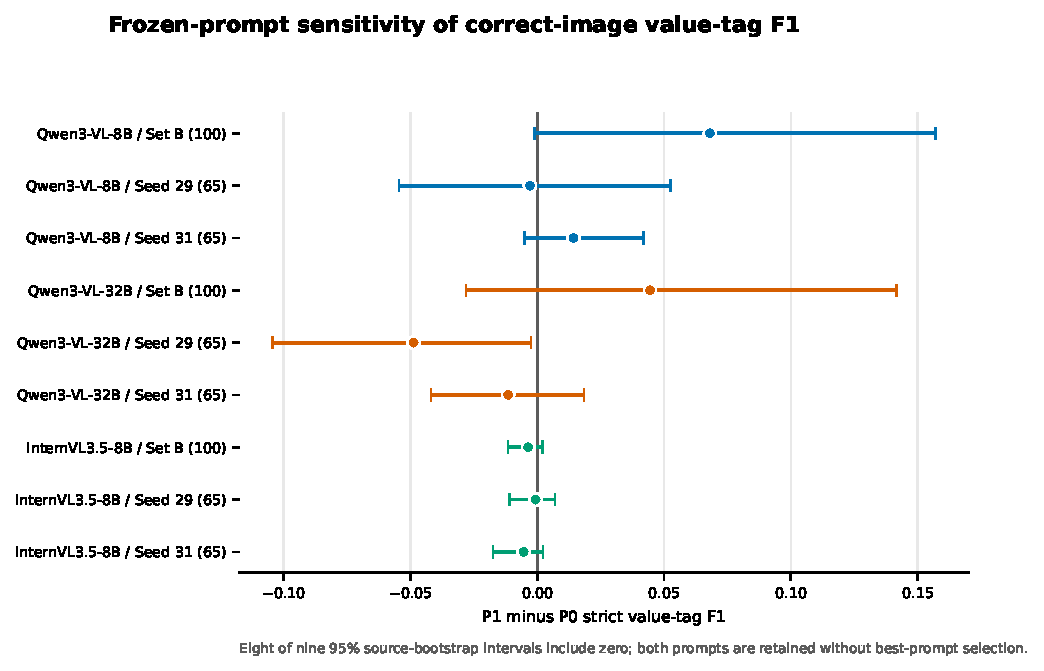
\includegraphics[width=\linewidth]{figure_s_v7_prompt_sensitivity.pdf}
\caption{Frozen-prompt sensitivity of correct-image strict value-tag F1.
Whiskers are 95\% intervals from 10,000 paired source-bootstrap replicates.}
\label{fig:s_v7_prompt}
\end{figure}

Table~\ref{tab:v7_tasks} preserves the all-task boundary: exact and aggregate
accuracy must not be substituted for the pooled tag-set F1 estimator used by
the qualified retrieval claim.

\begin{table}[H]
\centering
\caption{Correct-image strict accuracy by task under the frozen V7 configurations. Value F1 is pooled strict value-tag F1 and is not interchangeable with exact-set accuracy.}
\label{tab:v7_tasks}
\scriptsize
\setlength{\tabcolsep}{4pt}
\begin{tabular}{lllrrrrrr}
\toprule
Model & Subset & Prompt & Overall & Connectivity & Count & Spatial count & Value exact & Value F1 \\
\midrule
Qwen3-VL-8B & Set B (100) & P0 & 0.287 & 0.560 & 0.100 & 0.300 & 0.190 & 0.525 \\
Qwen3-VL-8B & Set B (100) & P1 & 0.295 & 0.570 & 0.110 & 0.310 & 0.190 & 0.593 \\
Qwen3-VL-8B & Seed 29 (65) & P0 & 0.315 & 0.569 & 0.108 & 0.323 & 0.262 & 0.659 \\
Qwen3-VL-8B & Seed 29 (65) & P1 & 0.273 & 0.554 & 0.092 & 0.246 & 0.200 & 0.656 \\
Qwen3-VL-8B & Seed 31 (65) & P0 & 0.258 & 0.523 & 0.046 & 0.215 & 0.246 & 0.616 \\
Qwen3-VL-8B & Seed 31 (65) & P1 & 0.265 & 0.538 & 0.062 & 0.215 & 0.246 & 0.630 \\
Qwen3-VL-32B & Set B (100) & P0 & 0.367 & 0.570 & 0.070 & 0.530 & 0.300 & 0.570 \\
Qwen3-VL-32B & Set B (100) & P1 & 0.365 & 0.570 & 0.070 & 0.530 & 0.290 & 0.614 \\
Qwen3-VL-32B & Seed 29 (65) & P0 & 0.396 & 0.554 & 0.062 & 0.554 & 0.415 & 0.736 \\
Qwen3-VL-32B & Seed 29 (65) & P1 & 0.388 & 0.554 & 0.062 & 0.554 & 0.385 & 0.687 \\
Qwen3-VL-32B & Seed 31 (65) & P0 & 0.327 & 0.523 & 0.062 & 0.446 & 0.277 & 0.657 \\
Qwen3-VL-32B & Seed 31 (65) & P1 & 0.327 & 0.523 & 0.062 & 0.446 & 0.277 & 0.645 \\
InternVL3.5-8B & Set B (100) & P0 & 0.033 & 0.000 & 0.110 & 0.020 & 0.000 & 0.013 \\
InternVL3.5-8B & Set B (100) & P1 & 0.080 & 0.150 & 0.140 & 0.030 & 0.000 & 0.009 \\
InternVL3.5-8B & Seed 29 (65) & P0 & 0.046 & 0.000 & 0.077 & 0.092 & 0.015 & 0.012 \\
InternVL3.5-8B & Seed 29 (65) & P1 & 0.058 & 0.092 & 0.077 & 0.046 & 0.015 & 0.012 \\
InternVL3.5-8B & Seed 31 (65) & P0 & 0.031 & 0.000 & 0.046 & 0.062 & 0.015 & 0.026 \\
InternVL3.5-8B & Seed 31 (65) & P1 & 0.058 & 0.123 & 0.077 & 0.015 & 0.015 & 0.020 \\
\bottomrule
\end{tabular}
\end{table}


The symbol-legend control preserves prototype crops, grid, font, dimensions,
and second-image count. Visible legend minus raw spatial-count accuracy is
+0.3100 [0.2200, 0.4100] at 768-side and +0.2400 [0.1500, 0.3400] at
3072-side. Correct numeric labels minus a layout-matched cyclic permutation
is +0.0000 [-0.0400, 0.0400] at both budgets. The visual context affects the
task, but the tested numeric mapping semantics do not show a detected effect.

\section*{S11. Artifact provenance and deterministic reproduction}

Run
\begin{quote}\ttfamily
python scripts/reproduce\_submission\_v6.py --root .
\end{quote}
from the repository root. The script re-scores immutable outputs, rebuilds the
v6 analysis and figures, runs unit and package checks, compiles manuscript and
supplement PDFs, and performs page-render validation. It does not rerun model
inference or retry the unavailable external-data branch.

The recovered V7 matrix is independently reproduced without new inference by
running
\begin{quote}\ttfamily
python scripts/reproduce\_rineng\_overnight\_v7.py --root .
\end{quote}
This command recomputes all 54 cell metrics, 36 paired effects and intervals,
and nine prompt-sensitivity intervals before rebuilding the V7 tables,
figures, and SHA-256 artifact manifest.

The principal v6 and V7 machine-readable artifacts are:
\begin{itemize}
\item \texttt{reports/generated/rineng\_revision\_analysis\_v6.json};
\item \texttt{reports/generated/rineng\_revision\_analysis\_v6.csv};
\item \texttt{reports/generated/rineng\_revision\_per\_source\_v6.csv};
\item \texttt{reports/generated/rineng\_revision\_error\_taxonomy\_v6.csv};
\item \texttt{paper/figures/figure\_metadata\_v6.json};
\item \texttt{reports/generated/rineng\_overnight\_v7\_score.json};
\item \texttt{reports/generated/rineng\_overnight\_v7\_validation.json};
\item \texttt{reports/RINENG\_OVERNIGHT\_V7\_ARTIFACT\_MANIFEST.json};
\item \texttt{paper/figures/figure\_metadata\_v7.json}.
\end{itemize}
The analysis JSON records the seven immutable input paths, byte sizes, and
SHA-256 hashes. The release archive additionally records dependency versions,
source manifests, raw model output identifiers and revisions, tests, and a
top-level SHA-256 inventory. GPU inference used NVIDIA H200 devices; model
weights are not redistributed.

The public release excludes author-side editorial prompts, model-review text,
private working notes, and submitter identity fields because none is required
to reproduce a result. Scorer-only references are included with explicit
separation from model-facing manifests. The public DOI/URL, author identities,
affiliations, CRediT roles, funding, competing-interest statement, and license
choice remain submitter-owned administrative fields.

\section*{S12. External-data boundary}

The attempted PID2Graph/OPEN100 acquisition did not yield a valid official
archive: the obtained file failed size, MD5, and ZIP-central-directory checks.
No archive member was extracted, no record was scored, and no cross-family
number is reported. The automated workflow therefore narrows the manuscript
claim rather than substituting simulated or unverifiable external evidence.

\end{document}
